
%% bare_conf.tex
%% V1.4b
%% 2015/08/26
%% by Michael Shell
%% See:
%% http://www.michaelshell.org/
%% for current contact information.
%%
%% This is a skeleton file demonstrating the use of IEEEtran.cls
%% (requires IEEEtran.cls version 1.8b or later) with an IEEE
%% conference paper.
%%
%% Support sites:
%% http://www.michaelshell.org/tex/ieeetran/
%% http://www.ctan.org/pkg/ieeetran
%% and
%% http://www.ieee.org/

%%*************************************************************************
%% Legal Notice:
%% This code is offered as-is without any warranty either expressed or
%% implied; without even the implied warranty of MERCHANTABILITY or
%% FITNESS FOR A PARTICULAR PURPOSE! 
%% User assumes all risk.
%% In no event shall the IEEE or any contributor to this code be liable for
%% any damages or losses, including, but not limited to, incidental,
%% consequential, or any other damages, resulting from the use or misuse
%% of any information contained here.
%%
%% All comments are the opinions of their respective authors and are not
%% necessarily endorsed by the IEEE.
%%
%% This work is distributed under the LaTeX Project Public License (LPPL)
%% ( http://www.latex-project.org/ ) version 1.3, and may be freely used,
%% distributed and modified. A copy of the LPPL, version 1.3, is included
%% in the base LaTeX documentation of all distributions of LaTeX released
%% 2003/12/01 or later.
%% Retain all contribution notices and credits.
%% ** Modified files should be clearly indicated as such, including  **
%% ** renaming them and changing author support contact information. **
%%*************************************************************************


% *** Authors should verify (and, if needed, correct) their LaTeX system  ***
% *** with the testflow diagnostic prior to trusting their LaTeX platform ***
% *** with production work. The IEEE's font choices and paper sizes can   ***
% *** trigger bugs that do not appear when using other class files.       ***                          ***
% The testflow support page is at:
% http://www.michaelshell.org/tex/testflow/

\documentclass[conference]{IEEEtran}
% Some Computer Society conferences also require the compsoc mode option,
% but others use the standard conference format.
%
% If IEEEtran.cls has not been installed into the LaTeX system files,
% manually specify the path to it like:
% \documentclass[conference]{../sty/IEEEtran}





% Some very useful LaTeX packages include:
% (uncomment the ones you want to load)


% *** MISC UTILITY PACKAGES ***
%
%\usepackage{ifpdf}
% Heiko Oberdiek's ifpdf.sty is very useful if you need conditional
% compilation based on whether the output is pdf or dvi.
% usage:
% \ifpdf
%   % pdf code
% \else
%   % dvi code
% \fi
% The latest version of ifpdf.sty can be obtained from:
% http://www.ctan.org/pkg/ifpdf
% Also, note that IEEEtran.cls V1.7 and later provides a builtin
% \ifCLASSINFOpdf conditional that works the same way.
% When switching from latex to pdflatex and vice-versa, the compiler may
% have to be run twice to clear warning/error messages.






% *** CITATION PACKAGES ***
%
%\usepackage{cite}
% cite.sty was written by Donald Arseneau
% V1.6 and later of IEEEtran pre-defines the format of the cite.sty package
% \cite{} output to follow that of the IEEE. Loading the cite package will
% result in citation numbers being automatically sorted and properly
% "compressed/ranged". e.g., [1], [9], [2], [7], [5], [6] without using
% cite.sty will become [1], [2], [5]--[7], [9] using cite.sty. cite.sty's
% \cite will automatically add leading space, if needed. Use cite.sty's
% noadjust option (cite.sty V3.8 and later) if you want to turn this off
% such as if a citation ever needs to be enclosed in parenthesis.
% cite.sty is already installed on most LaTeX systems. Be sure and use
% version 5.0 (2009-03-20) and later if using hyperref.sty.
% The latest version can be obtained at:
% http://www.ctan.org/pkg/cite
% The documentation is contained in the cite.sty file itself.






% *** GRAPHICS RELATED PACKAGES ***
%
\ifCLASSINFOpdf
  % \usepackage[pdftex]{graphicx}
  % declare the path(s) where your graphic files are
  % \graphicspath{{../pdf/}{../jpeg/}}
  % and their extensions so you won't have to specify these with
  % every instance of \includegraphics
  % \DeclareGraphicsExtensions{.pdf,.jpeg,.png}
\else
  % or other class option (dvipsone, dvipdf, if not using dvips). graphicx
  % will default to the driver specified in the system graphics.cfg if no
  % driver is specified.
  % \usepackage[dvips]{graphicx}
  % declare the path(s) where your graphic files are
  % \graphicspath{{../eps/}}
  % and their extensions so you won't have to specify these with
  % every instance of \includegraphics
  % \DeclareGraphicsExtensions{.eps}
\fi
% graphicx was written by David Carlisle and Sebastian Rahtz. It is
% required if you want graphics, photos, etc. graphicx.sty is already
% installed on most LaTeX systems. The latest version and documentation
% can be obtained at: 
% http://www.ctan.org/pkg/graphicx
% Another good source of documentation is "Using Imported Graphics in
% LaTeX2e" by Keith Reckdahl which can be found at:
% http://www.ctan.org/pkg/epslatex
%
% latex, and pdflatex in dvi mode, support graphics in encapsulated
% postscript (.eps) format. pdflatex in pdf mode supports graphics
% in .pdf, .jpeg, .png and .mps (metapost) formats. Users should ensure
% that all non-photo figures use a vector format (.eps, .pdf, .mps) and
% not a bitmapped formats (.jpeg, .png). The IEEE frowns on bitmapped formats
% which can result in "jaggedy"/blurry rendering of lines and letters as
% well as large increases in file sizes.
%
% You can find documentation about the pdfTeX application at:
% http://www.tug.org/applications/pdftex





% *** MATH PACKAGES ***
%
%\usepackage{amsmath}
% A popular package from the American Mathematical Society that provides
% many useful and powerful commands for dealing with mathematics.
%
% Note that the amsmath package sets \interdisplaylinepenalty to 10000
% thus preventing page breaks from occurring within multiline equations. Use:
%\interdisplaylinepenalty=2500
% after loading amsmath to restore such page breaks as IEEEtran.cls normally
% does. amsmath.sty is already installed on most LaTeX systems. The latest
% version and documentation can be obtained at:
% http://www.ctan.org/pkg/amsmath





% *** SPECIALIZED LIST PACKAGES ***
%
%\usepackage{algorithmic}
% algorithmic.sty was written by Peter Williams and Rogerio Brito.
% This package provides an algorithmic environment fo describing algorithms.
% You can use the algorithmic environment in-text or within a figure
% environment to provide for a floating algorithm. Do NOT use the algorithm
% floating environment provided by algorithm.sty (by the same authors) or
% algorithm2e.sty (by Christophe Fiorio) as the IEEE does not use dedicated
% algorithm float types and packages that provide these will not provide
% correct IEEE style captions. The latest version and documentation of
% algorithmic.sty can be obtained at:
% http://www.ctan.org/pkg/algorithms
% Also of interest may be the (relatively newer and more customizable)
% algorithmicx.sty package by Szasz Janos:
% http://www.ctan.org/pkg/algorithmicx




% *** ALIGNMENT PACKAGES ***
%
%\usepackage{array}
% Frank Mittelbach's and David Carlisle's array.sty patches and improves
% the standard LaTeX2e array and tabular environments to provide better
% appearance and additional user controls. As the default LaTeX2e table
% generation code is lacking to the point of almost being broken with
% respect to the quality of the end results, all users are strongly
% advised to use an enhanced (at the very least that provided by array.sty)
% set of table tools. array.sty is already installed on most systems. The
% latest version and documentation can be obtained at:
% http://www.ctan.org/pkg/array


% IEEEtran contains the IEEEeqnarray family of commands that can be used to
% generate multiline equations as well as matrices, tables, etc., of high
% quality.




% *** SUBFIGURE PACKAGES ***
%\ifCLASSOPTIONcompsoc
%  \usepackage[caption=false,font=normalsize,labelfont=sf,textfont=sf]{subfig}
%\else
%  \usepackage[caption=false,font=footnotesize]{subfig}
%\fi
% subfig.sty, written by Steven Douglas Cochran, is the modern replacement
% for subfigure.sty, the latter of which is no longer maintained and is
% incompatible with some LaTeX packages including fixltx2e. However,
% subfig.sty requires and automatically loads Axel Sommerfeldt's caption.sty
% which will override IEEEtran.cls' handling of captions and this will result
% in non-IEEE style figure/table captions. To prevent this problem, be sure
% and invoke subfig.sty's "caption=false" package option (available since
% subfig.sty version 1.3, 2005/06/28) as this is will preserve IEEEtran.cls
% handling of captions.
% Note that the Computer Society format requires a larger sans serif font
% than the serif footnote size font used in traditional IEEE formatting
% and thus the need to invoke different subfig.sty package options depending
% on whether compsoc mode has been enabled.
%
% The latest version and documentation of subfig.sty can be obtained at:
% http://www.ctan.org/pkg/subfig




% *** FLOAT PACKAGES ***
%
%\usepackage{fixltx2e}
% fixltx2e, the successor to the earlier fix2col.sty, was written by
% Frank Mittelbach and David Carlisle. This package corrects a few problems
% in the LaTeX2e kernel, the most notable of which is that in current
% LaTeX2e releases, the ordering of single and double column floats is not
% guaranteed to be preserved. Thus, an unpatched LaTeX2e can allow a
% single column figure to be placed prior to an earlier double column
% figure.
% Be aware that LaTeX2e kernels dated 2015 and later have fixltx2e.sty's
% corrections already built into the system in which case a warning will
% be issued if an attempt is made to load fixltx2e.sty as it is no longer
% needed.
% The latest version and documentation can be found at:
% http://www.ctan.org/pkg/fixltx2e


%\usepackage{stfloats}
% stfloats.sty was written by Sigitas Tolusis. This package gives LaTeX2e
% the ability to do double column floats at the bottom of the page as well
% as the top. (e.g., "\begin{figure*}[!b]" is not normally possible in
% LaTeX2e). It also provides a command:
%\fnbelowfloat
% to enable the placement of footnotes below bottom floats (the standard
% LaTeX2e kernel puts them above bottom floats). This is an invasive package
% which rewrites many portions of the LaTeX2e float routines. It may not work
% with other packages that modify the LaTeX2e float routines. The latest
% version and documentation can be obtained at:
% http://www.ctan.org/pkg/stfloats
% Do not use the stfloats baselinefloat ability as the IEEE does not allow
% \baselineskip to stretch. Authors submitting work to the IEEE should note
% that the IEEE rarely uses double column equations and that authors should try
% to avoid such use. Do not be tempted to use the cuted.sty or midfloat.sty
% packages (also by Sigitas Tolusis) as the IEEE does not format its papers in
% such ways.
% Do not attempt to use stfloats with fixltx2e as they are incompatible.
% Instead, use Morten Hogholm'a dblfloatfix which combines the features
% of both fixltx2e and stfloats:
%
% \usepackage{dblfloatfix}
% The latest version can be found at:
% http://www.ctan.org/pkg/dblfloatfix




% *** PDF, URL AND HYPERLINK PACKAGES ***
%
%\usepackage{url}
% url.sty was written by Donald Arseneau. It provides better support for
% handling and breaking URLs. url.sty is already installed on most LaTeX
% systems. The latest version and documentation can be obtained at:
% http://www.ctan.org/pkg/url
% Basically, \url{my_url_here}.




% *** Do not adjust lengths that control margins, column widths, etc. ***
% *** Do not use packages that alter fonts (such as pslatex).         ***
% There should be no need to do such things with IEEEtran.cls V1.6 and later.
% (Unless specifically asked to do so by the journal or conference you plan
% to submit to, of course. )


% correct bad hyphenation here
\hyphenation{op-tical net-works semi-conduc-tor}

\usepackage{tikz}
\usetikzlibrary{arrows,positioning,automata}
\usepackage[noend]{algpseudocode}
\usepackage{algorithm}
\usepackage{enumitem, kantlipsum}

\begin{document}
%
% paper title
% Titles are generally capitalized except for words such as a, an, and, as,
% at, but, by, for, in, nor, of, on, or, the, to and up, which are usually
% not capitalized unless they are the first or last word of the title.
% Linebreaks \\ can be used within to get better formatting as desired.
% Do not put math or special symbols in the title.

% \title{Affect-Driven Action Selection in\\Human-Robot Collaboration}
% \title{Human-Robot Collaboration:\\How Emotions Help to Do the Right Thing?}
\title{{\fontsize{19}{20}\selectfont Impact of Affective Appraisal on
Collaborative Goal Management:\\How My Robot Shares My Worries}}

% author names and affiliations
% use a multiple column layout for up to three different
% affiliations

% \author{\IEEEauthorblockN{Mahni Shayganfar and Charles Rich and Candace
% L. Sidner} 
% \IEEEauthorblockA{Fuller Laboratories\\
% Computer Science Department\\
% Worcester Polytechnic Institute\\
% Worcester, Massachusetts 01609-2280\\
% mshayganfar $|$ rich $|$ sidner@wpi.edu}}

\author{Anonymous}

% conference papers do not typically use \thanks and this command
% is locked out in conference mode. If really needed, such as for
% the acknowledgment of grants, issue a \IEEEoverridecommandlockouts
% after \documentclass

% for over three affiliations, or if they all won't fit within the width
% of the page, use this alternative format:
% 
%\author{\IEEEauthorblockN{Michael Shell\IEEEauthorrefmark{1},
%Homer Simpson\IEEEauthorrefmark{2},
%James Kirk\IEEEauthorrefmark{3}, 
%Montgomery Scott\IEEEauthorrefmark{3} and
%Eldon Tyrell\IEEEauthorrefmark{4}}
%\IEEEauthorblockA{\IEEEauthorrefmark{1}School of Electrical and Computer Engineering\\
%Georgia Institute of Technology,
%Atlanta, Georgia 30332--0250\\ Email: see http://www.michaelshell.org/contact.html}
%\IEEEauthorblockA{\IEEEauthorrefmark{2}Twentieth Century Fox, Springfield, USA\\
%Email: homer@thesimpsons.com}
%\IEEEauthorblockA{\IEEEauthorrefmark{3}Starfleet Academy, San Francisco, California 96678-2391\\
%Telephone: (800) 555--1212, Fax: (888) 555--1212}
%\IEEEauthorblockA{\IEEEauthorrefmark{4}Tyrell Inc., 123 Replicant Street, Los Angeles, California 90210--4321}}




% use for special paper notices
%\IEEEspecialpapernotice{(Invited Paper)}




% make the title area
\maketitle

% As a general rule, do not put math, special symbols or citations
% in the abstract
\begin{abstract}
A collaborative robot needs to be able to regulate and manage shared goals
during collaboration. Emotion has a crucial influence on the goal management
process. In this paper, we provide a cost function that we use to choose the
goal in the shared plan with the lowest cost value out of a set of alternative
goals. This cost function provides the cost value a) based on the goal
attributes we consider in our framework, b) with respect to the reverse
appraisal of the percived emotion, and c) the appraisal of the collaborative
environment.
\end{abstract}

% no keywords




% For peer review papers, you can put extra information on the cover
% page as needed:
% \ifCLASSOPTIONpeerreview
% \begin{center} \bfseries EDICS Category: 3-BBND \end{center}
% \fi
%
% For peerreview papers, this IEEEtran command inserts a page break and
% creates the second title. It will be ignored for other modes.
\IEEEpeerreviewmaketitle

\vspace*{-2mm}
\section{Introduction}

% Cognitive architectures involve various components and processes to provide
% cognitive functions to intelligent agents. All these cognitive functions
% ultimately serve the agents what goal to pursue next. However, there
% should be a process to provide dynamic adjustments in goal priority in response
% to internal and external changes.

Goals represent an important part of the context during collaboration. However,
not all goals are appropriate to pursue, depending on conditions. In fact, it
can be destructive for a collaboration to pursue a good goal in a wrong context.
Therefore, a collaborative robot must be able to manage shared goals during
collaboration. The goal management process provides a critical influence on a
collaborative robot's behavior by maintaining or shifting the focus of attention
to an appropriate goal based on the collaboration status.

% Most of the times, emotions are the repercussions of the changes in the
% environment.

Changes in a collaboration environment alter the balance of alternative goals.
These changes can reflect the collaborators' internal changes, and the influence
of their actions. In a collaboration environment, emotions represent the outcome
of underlying internal mental processes of the collaborators. Emotions have
different functions \cite{scheutz:architectural-action-selection}. These
functions, e.g., \textit{goal management}, help one to communicate and/or
regulate internal changes as well as changes in the environment. Goal-oriented
emotions such as anger, frustration and worriedness, constitute the mental
processes specifically influenced by one's internal goals. Therefore, reverse
appraisal \cite{gratch:reverse-appraisal} of the collaborator's perceived
emotion can impact regulation of the robot's active goals during collaboration.
Furthermore, the appraisal of the individual alternative goals provides a
context-dependent assessment of these goals. Hence, we use both appraisal and
reverse appraisal in our goal management process.

% The evaluative aspect of the affective appraisal processes has a
% key role in differentiating between available goals.

\vspace*{-2mm}
\section{Contribution}

Here, we focus on a small part of a larger architecture framework built based on
our \textit{Affective Motivational Collaboration Theory}
\cite{shayganfar:amct-symbiotic}. We introduce our goal management process based
on a cost function including the influence of affective appraisal and reverse
appraisal processes. Goal management is a crucial part of our investigation of
the reciprocal influence of appraisal on a collaboration structure (see Figure
\ref{fig:actionSelection}).

\begin{figure}[tbh]
  \centering
  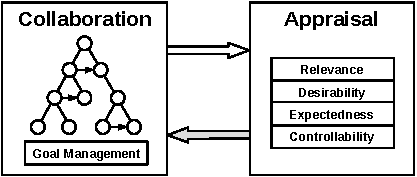
\includegraphics[width=0.36\textwidth]{figure/ActionSelection-croped.pdf}
  \vspace*{-2mm}
  \caption{{\fontsize{9}{9}\selectfont Reciprocal influence of Collaboration
  and Appraisal mechanisms in our framework.}}
  \label{fig:actionSelection}
  \vspace*{-7mm}
\end{figure}

We have investigated the influence of a collaboration structure on
appraisal processes, and implemented distinct algorithms for different
appraisal processes for a collaborative robot \cite{shayganfar:appraisal}.
According to the appraisal theory, the outcome of these processes are separable
antecedents of emotion with which the robot evaluates the environment. Our
appraisal variables included: a) \textit{relevance} used to measure the
significance of an event for the robot, b) \textit{desirability} to characterize
the value of an event to the robot in terms of whether the event facilitates or
thwarts the collaboration goal, c) \textit{expectedness} and d)
\textit{controllability} (the last two appraisal variables are beyond the scope
of this paper). The outcome of each appraisal process is a specific value for
the corresponding appraisal variable. The vector containing these appraisal
variables can be mapped to a particular emotion instance at each point in time.
For instance, a \textit{relevant, undesirable, expected}, and
\textit{uncontrollable} event can elicit \textit{anger} in an individual.
However, it is not the actual emotion instance that is important for us. In
fact, it is a) the functions of emotions in a social setting, i.e., \textit{goal
management}, and b) the meaning of the collabrator's perceived emotion in
collaboration context.

A collaboration structure provides a hierarchy and constraints of the shared
goals in the form of a shared plan (Figure \ref{fig:taskModel}) which contains
both the robot and the human collaborator's goals. The robot pursues the goals
for which the robot is responsible in the shared plan. However, there can be
several goals available for the robot to pursue at each point in time during
collaboration. In other words, any ``live'' goal can be pursued by the robot. A
goal is live if all of its \textit{predecessors} are achieved and all of its
\textit{preconditions} are satisfied. Therefore, a collaborative robot requires
a mechanism to choose between a set of live goals. We believe appraisal
processes are crucial to choose between the available live goals; since the
appraisals are the immediate outcome of the robot's assessment of the
collaboration environment.

\begin{figure}[tbh]
  \centering
  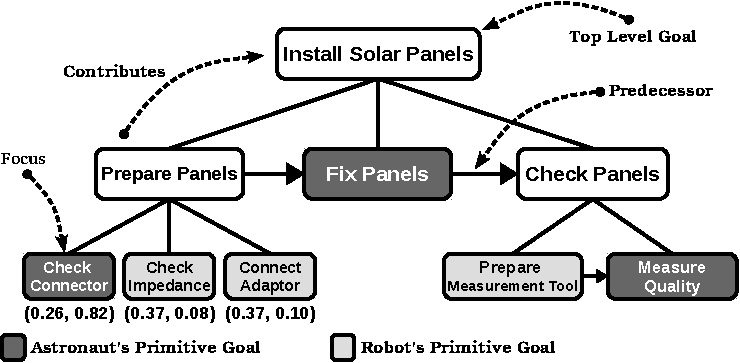
\includegraphics[width=0.44\textwidth]{figure/collaborationStructure-croped.pdf}
  \vspace*{-3mm}
  \caption{{\fontsize{9}{9}\selectfont Astronaut-robot collaboraiton structure
  (shared plan).}}
  \label{fig:taskModel}
  \vspace*{-6mm}
\end{figure}

For instance, Figure \ref{fig:taskModel} shows a nonprimitive ``Prepare Panels''
goal which contains three primitive goals. These primitive goals do not have any
temporal constraint between them. Therefore, if ``Prepare Panels'' is live, its
primitive goals can be pursued by the responsible agent. In this example, the
astronaut is responsible for the primitive goal ``Check Connector''; the robot
is responsible for the remaining two primitive goals. According to the
collaboration mechanism in our overall framework, ``Check Connector'' is in
focus, with the astronaut pursuing this goal. Suddenly, the astronaut tells the
robot that the connector is broken and she is \textit{worried} about failure of
the overall goal.

Equation \ref{eqn:cost} shows our general cost function we use to calculate the
cost of each individual potential goal. The base in the equation is considered
to calculate the cost of pursuing any given goal. There are three different
functions used to calculate the cost, including \textit{proximity} of a goal
$P(g)$, \textit{difficulty} of a goal $D(g)$, and \textit{specificity} of a
goal $S(g)$. The details about these functions are provided in equations
\ref{eqn:proximity} to \ref{eqn:specificity}. The exponent part of our cost
function is considered to capture a) the influence of human's emotional instance
on the cost, and b) the influece of self appraisal of any given goal. The
$R_h\in[0,1]$ and $D_h\in[-1,1]$  are \textit{relevance} and
\textit{desirability} values respectively, which will be attained based on the
reverse appraisal of the human's perceived emotion. For instance, if the
astronaut is frustrated $D_h$ obtains a negative value (depending on how
undesirable is the event according to reverse appraisal), and $R_h$ will be 1
for the active goal and its value descends to 0 for other live goals depending
on their distance to the active goal in the shared plan. $R_r\in[0,1]$ and
$D_r\in[-1,1]$ are also \textit{relevance} and \textit{desirability} values.
However, the self appraisal functions provide these values for all of the live
goals. For instance, for the active goal for which the astronuat was frustrated,
$D_r$ can be a positive value (depending on the self's desirability appraisal
function); $R_r$ can be 1, since the active goal is \textit{relevant} for the
robot. These values will change for the other live goals depending on how
\textit{relevant} they are with respect to the collaboration status. Finally,
$C\in[1,\infty]$ is a constant used to control the influence of affect on cost
value. It has negative sign since \textit{undesirablity} (negative values)
should increase the cost. $\alpha\in[1,\infty]$ is another constant used to
control the importance of reverse appraisal relative to self appraisal.

\vspace*{-4mm}
\begin{equation}
Cost(g) = \left(\frac{P(g)\times D(g)}{S(g)+1}\right)^{-C[(R_r+1)D_r + \alpha
(R_h+1)D_h]}
\label{eqn:cost}
\end{equation}

The \textit{proximity} of a goal indicates how far the goal is from the current
active goal in the shared plan. It is calculated by the distance function
(Equation \ref{eqn:proximity}) which returns the number of edges between the
current active goal $g_{_{act}}$, and the given goal $g$ in the shared plan.

\vspace*{-3mm}
\begin{equation}
P(g) =  distance(g_{_{act}},g)
\label{eqn:proximity}
\end{equation}

The \textit{difficulty} of a goal is a function of three parameters (Equation
\ref{eqn:difficulty}) which consider the difficulty based on a) topology of the
shared plan tree (domain independent), and b) the amount of effort required to
pursue a given goal (domain dependent). The $\sum pred_e(g)$ is the sum of
efforts that all the \textit{predecessors} of a given goal $g$ require. The
$\sum desc_e(g)$ is the sum of efforts that all the \textit{descendants} of a
given goal $g$ require. The effort values represent the amount of effort for the
goals with respect to the domain. The $H(g)$ is the height of the given goal $g$
and it is important since a goal with higher height value (longest path from the
goal to a leaf; a primitive goal) makes the collaboration more difficult than a
goal with shorter height.

\vspace*{-7mm}
\begin{equation}
D(g) = \Big(H(g)+1\Big)\times\left[\sum\limits_{m=0}^{M} pred_e(g) +
\sum\limits_{n=0}^{N} desc_e(g)\right]
\label{eqn:difficulty}
\end{equation}

The \textit{specificity} of a goal is the function of \textit{depth} (distance
from the root) and \textit{degree} (number of children) of a given goal $g$. The
first number primitive goal (root) is the least specific goal, and the
primitives (leaves) are the most specific goals.

\vspace*{-3mm}
\begin{equation}
S(g) = \frac{depth(g)}{degree(g)+1}
\label{eqn:specificity}
\end{equation}

\vspace*{-1mm}
The tuples below the goals in Figure \ref{fig:taskModel} indicate the cost value
of each goal. The first number in each tuple is the cost value without the
influence of the affective part of the cost function, i.e., the exponent is
equal to 1 in Equation \ref{eqn:cost}. The second number of each tuple indicates
the value of the cost including the influence of affective appraisal and the
astronaut's perceived emotion.

The robot perceives and interprets the astronaut's negative emotion using
reverse appraisal (the details about reverse appraisal process in our framework
is beyond the scope of this paper). Then, the robot evaluates the cost function
for the current and the live goals. The astronaut's negative emotion increases
the cost of pursuing the current goal, and also affects two other primitive live
goals under the same parent. Therefore, instead of insisting on pursuing the
same blocked goal which has caused the astronaut's negative emotion, the robot
acknowledges the astronaut's emotion. The robot's behavior mitigates the
astronaut negative emotion allowing the robot to pursue another live goal
``Coonect Adaptor" which has a lower cost with respect to the collaboration
status. The details about the robot's behavior is beyond the scope of this
paper.

% An example of a floating figure using the graphicx package.
% Note that \label must occur AFTER (or within) \caption.
% For figures, \caption should occur after the \includegraphics.
% Note that IEEEtran v1.7 and later has special internal code that
% is designed to preserve the operation of \label within \caption
% even when the captionsoff option is in effect. However, because
% of issues like this, it may be the safest practice to put all your
% \label just after \caption rather than within \caption{}.
%
% Reminder: the "draftcls" or "draftclsnofoot", not "draft", class
% option should be used if it is desired that the figures are to be
% displayed while in draft mode.
%
%\begin{figure}[!t]
%\centering
%\includegraphics[width=2.5in]{myfigure}
% where an .eps filename suffix will be assumed under latex, 
% and a .pdf suffix will be assumed for pdflatex; or what has been declared
% via \DeclareGraphicsExtensions.
%\caption{Simulation results for the network.}
%\label{fig_sim}
%\end{figure}

% Note that the IEEE typically puts floats only at the top, even when this
% results in a large percentage of a column being occupied by floats.


% An example of a double column floating figure using two subfigures.
% (The subfig.sty package must be loaded for this to work.)
% The subfigure \label commands are set within each subfloat command,
% and the \label for the overall figure must come after \caption.
% \hfil is used as a separator to get equal spacing.
% Watch out that the combined width of all the subfigures on a 
% line do not exceed the text width or a line break will occur.
%
%\begin{figure*}[!t]
%\centering
%\subfloat[Case I]{\includegraphics[width=2.5in]{box}%
%\label{fig_first_case}}
%\hfil
%\subfloat[Case II]{\includegraphics[width=2.5in]{box}%
%\label{fig_second_case}}
%\caption{Simulation results for the network.}
%\label{fig_sim}
%\end{figure*}
%
% Note that often IEEE papers with subfigures do not employ subfigure
% captions (using the optional argument to \subfloat[]), but instead will
% reference/describe all of them (a), (b), etc., within the main caption.
% Be aware that for subfig.sty to generate the (a), (b), etc., subfigure
% labels, the optional argument to \subfloat must be present. If a
% subcaption is not desired, just leave its contents blank,
% e.g., \subfloat[].


% An example of a floating table. Note that, for IEEE style tables, the
% \caption command should come BEFORE the table and, given that table
% captions serve much like titles, are usually capitalized except for words
% such as a, an, and, as, at, but, by, for, in, nor, of, on, or, the, to
% and up, which are usually not capitalized unless they are the first or
% last word of the caption. Table text will default to \footnotesize as
% the IEEE normally uses this smaller font for tables.
% The \label must come after \caption as always.
%
%\begin{table}[!t]
%% increase table row spacing, adjust to taste
%\renewcommand{\arraystretch}{1.3}
% if using array.sty, it might be a good idea to tweak the value of
% \extrarowheight as needed to properly center the text within the cells
%\caption{An Example of a Table}
%\label{table_example}
%\centering
%% Some packages, such as MDW tools, offer better commands for making tables
%% than the plain LaTeX2e tabular which is used here.
%\begin{tabular}{|c||c|}
%\hline
%One & Two\\
%\hline
%Three & Four\\
%\hline
%\end{tabular}
%\end{table}


% Note that the IEEE does not put floats in the very first column
% - or typically anywhere on the first page for that matter. Also,
% in-text middle ("here") positioning is typically not used, but it
% is allowed and encouraged for Computer Society conferences (but
% not Computer Society journals). Most IEEE journals/conferences use
% top floats exclusively. 
% Note that, LaTeX2e, unlike IEEE journals/conferences, places
% footnotes above bottom floats. This can be corrected via the
% \fnbelowfloat command of the stfloats package.

\vspace*{-2mm}
\section{Conclusion}

We use our proposed cost function in our goal management algorithm to be able to
integrate affective appraisal into the collaboration mechanism in our framework.
We will evaluate our cost function through conducting a user study to compare
our results with humans' responses. We will continue to implement other parts of
our framework, including action selection and motivation processes.
\vspace*{-2mm}

% conference papers do not normally have an appendix

% use section* for acknowledgment
% \section*{Acknowledgment}
% {\fontsize{8.2}{9}\selectfont This work is supported by the National Science
% Foundation under award IIS-1012083. Any opinions, findings, and conclusions
% expressed in this material are those of the authors and do not necessarily
% reflect the views of the National Science Foundation.}

% trigger a \newpage just before the given reference
% number - used to balance the columns on the last page
% adjust value as needed - may need to be readjusted if
% the document is modified later
%\IEEEtriggeratref{8}
% The "triggered" command can be changed if desired:
%\IEEEtriggercmd{\enlargethispage{-5in}}

% references section

% can use a bibliography generated by BibTeX as a .bbl file
% BibTeX documentation can be easily obtained at:
% http://mirror.ctan.org/biblio/bibtex/contrib/doc/
% The IEEEtran BibTeX style support page is at:
% http://www.michaelshell.org/tex/ieeetran/bibtex/
%\bibliographystyle{IEEEtran}
% argument is your BibTeX string definitions and bibliography database(s)
%\bibliography{IEEEabrv,../bib/paper}
%
% <OR> manually copy in the resultant .bbl file
% set second argument of \begin to the number of references
% (used to reserve space for the reference number labels box)
\bibliographystyle{IEEEtran}
\bibliography{mshayganfar.bib}

% that's all folks
\end{document}